\documentclass[a4paper,ngerman,12pt]{exam}
\usepackage{babel}
\usepackage[utf8]{inputenc}
\usepackage[T1]{fontenc}
\usepackage{graphicx}
\usepackage{algpseudocode}
\usepackage{geometry}
\usepackage{csquotes} % Anführungszeichen
\usepackage{paralist} % kompakte Aufzählungen
\usepackage{textcomp,tikz} %diverses
\usepackage{amsmath,amssymb,amstext,amsthm}
\usepackage{listings}
\usepackage{mathtools}
\usepackage{mdframed} % Boxen
\usepackage{float}
\usepackage{tikz}
\usetikzlibrary{calc}
\usetikzlibrary{shapes, arrows, positioning,automata}

\geometry{a4paper, top=3cm, left=2.7cm, right=2.7cm, bottom=2.5cm}
\pagestyle{plain}
\renewcommand{\solutiontitle}{\noindent\textbf{Lösung:}\enspace}
\DeclarePairedDelimiter\ceil{\lceil}{\rceil}
\DeclarePairedDelimiter\floor{\lfloor}{\rfloor}

%\printanswers

\begin{document}
\noindent Theoretische Informatik \hfill Gruppe 8 \\
\mbox{}\hfill Loris Reiff
\begin{center}
  \bfseries\Large
  Midterm Vorbereitung \ifprintanswers
  -- Lösungen
\fi
\end{center}


\begin{questions}
\question
  \begin{parts}
    \part
  Sei $w = (10)^{2^{2^{n^2 + 1}}} \in \{0,1\}^*$ für alle $n \in \mathbb{N}$.
  Zeige, dass eine Konstante $d \in \mathbb{N}$ existiert, so dass für alle
  $n \in \mathbb{N}$ gilt, dass
  \begin{align*}
    K(w_n) &\leq \frac{1}{2}\log_2 (\log_2 \left(\log_2|w_n| - 1\right) - 1) + d
  \end{align*}

\begin{solutionorbox}
  Wir geben zunächst für jedes $n\in \mathbb{N}$ ein Programm an, welches
  $w_n$ erzeugt
\begin{lstlisting}[language=Pascal, mathescape=true]
begin
  x := $n$;
  x := 2^(2^(x*x + 1));
  for i:=1 to x do
    write(10);
end;
\end{lstlisting}
Der einzige Teil des Maschinencodes dieses Programms, der von $w_n$ abhängt, ist
die Darstellung von $n$ in der zweiten Zeile.
Der restliche Programmcode hat eine konstante Länge.
Also ist die binäre Länge dieses Programms $\ceil{\log_2 (n + 1)} + c$ für
eine Konstante c.

Damit lässt sich die Kolmogorov-Komplexität von $w_n$ von oben abschätzen durch
  \begin{align*}
    K(w_n) \leq \ceil{\log_2 (n + 1)} + c \leq \log_2 (n) + c + 1
  \end{align*}
  Die Länge von $w_n$ ist: 
  \begin{align*}
    |w_n| = 2\cdot 2^{2^{n^2 + 1}}
    &\iff \log_2 |w_n| - 1 = 2^{n^2+1}\\
    &\iff \log_2 \left(\log_2 |w_n| - 1\right) = n^2 + 1 \\
    &\iff \sqrt{\log_2 \left(\log_2|w_n| - 1\right) - 1} = n
  \end{align*}
  somit
  \begin{align*}
    K(w_n) &\leq \log_2 \sqrt{\log_2 \left(\log_2|w_n| - 1\right) - 1} + c + 1 \\
      &\leq \frac{1}{2}\log_2 (\log_2 \left(\log_2|w_n| - 1\right) - 1) + d
  \end{align*}
  mit $d = c + 1$.
    \end{solutionorbox}

\ifprintanswers
\newpage
\fi
    \part
    Wir betrachten die Sprache
    \begin{align*}
      L_1 &= \{101^i0^j1^k \mid i + k = j, \text{mit } i,j,k \in \mathbb{N}\}
    \end{align*}
    Sei $w_n$ das kanonisch $n$-te Wort in $L_1$. Zeige, dass es eine Konstante
    $c \in \mathbb{N}$ gibt, so dass für alle $n \in \mathbb{N}$ gilt:
    \begin{align*}
      K(w_n) \leq 2\cdot \log_2\left(|w_n|\right) + c
    \end{align*}
    \begin{solutionorbox}
      Es gibt offensichtlich ein Programm $A$, welches für ein Wort
      $w \in \Sigma_{\text{bool}}^*$
      entscheidet, ob
      $w \in L_1$ oder $w \not\in L_1$.
      Nach Satz 2.2 aus dem Buch gilt für das $n$-te kanonische Wort
      der Sprache $L_1$ somit
      \begin{align*}
        K(w_n) \leq \ceil{\log_2(n+1)} + c
      \end{align*}
      für eine von $n$ unabhängiger Konstante. Bemerke jedes Wort in $L_1$ hat
      eine gerade Länge und ist länger als 1.
      Des weiteren sehen wir, dass es $j+1$ verschiedene Wörter der Länge
      $2j+2$ in $L_1$ gibt mit $j \in \mathbb{N}$. Wir können also die
      Anzahl aller Wörter mit Länge $\leq 2j+2$, wie folgt abschätzen
      \begin{align*}
        \sum_{i=0}^j (i+1) &= j + 1 +\sum_{i=1}^j i \\
          &= j + 1 + \frac{j(j+1)}{2} \leq (2j)^2 -1
      \end{align*}
      für alle $j \geq 1$. Das heisst, es gibt maximal $(2j)^2 -1$ Wörter
      der Länge höchstens $2j+2$. Wenn wir $n = (2j)^2$ setzen, folgt, dass das
      die Wörter $w_n$ eine Länge grösser $2j + 3$ haben.
      Somit $|w_n| \geq 2j + 3 = \sqrt{n} + 3 \geq \sqrt{n}$.
      Nun können wir die Behauptung einfach folgern
      \begin{align*}
        K(w_n) &\leq \ceil{\log_2(n+1)} + c \\
        &\leq \log_2(n+1) + c' \\
        &\leq \log_2(|w_n|^2) + c' \\
        &\leq 2\log_2(|w_n|^2) + c'
      \end{align*}
      für eine Konstante $c'$.
    \end{solutionorbox}
  \end{parts}

\ifprintanswers
\newpage
\fi

\question
  \begin{parts}
    \part Entwerfe einen endlichen Automaten (in Diagrammdarstellung) für die Sprache
    \begin{align*}
      L_2 = \{w \in \{0,1\}^* \mid |w_n| \text{ ist gerade und Nummer}(w) \equiv_3 0
         \text{ und } w \text{ ist die} \\ \text{kürzeste Binärdarstellung für Nummer}(w)\}
    \end{align*}
    Begründe deinen Entwurf.
    \begin{solutionorbox}
      Die Sprache wird von folgendem Automaten akzeptiert \\
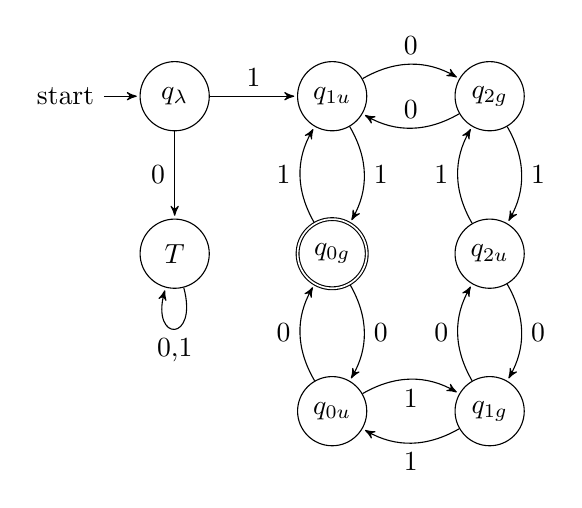
\begin{tikzpicture}[->,>=stealth',shorten >=1pt,auto,node distance=2cm]
  \node[initial, state]   (q0)                {$q_\lambda$};
  \node[state]            (T)   [below of=q0]  {$T$};
  \node[state]            (q1u) [right of=q0]  {$q_{1u}$};
  \node[state]            (q2g) [right of=q1u] {$q_{2g}$};
  \node[state,accepting]  (q0g) [below of=q1u] {$q_{0g}$};
  \node[state]            (q0u) [below of=q0g] {$q_{0u}$};
  \node[state]            (q2u) [below of=q2g] {$q_{2u}$};
  \node[state]            (q1g) [below of=q2u] {$q_{1g}$};

  \path[->]
        (q0)  edge []          node [left]  {0} (T)
              edge []          node [above] {1} (q1u)
        (q1u) edge [bend left] node [above] {0} (q2g)
              edge [bend left] node [right] {1} (q0g)
        (q2g) edge [bend left] node [above] {0} (q1u)
              edge [bend left] node [right] {1} (q2u)
        (q2u) edge [bend left] node [right] {0} (q1g)
              edge [bend left] node [left] {1} (q2g)
        (q1g) edge [bend left] node [left] {0} (q2u)
              edge [bend left] node [below] {1} (q0u)
        (q0u) edge [bend left] node [left] {0} (q0g)
              edge [bend left] node [below] {1} (q1g)
        (q0g) edge [bend left] node [right] {0} (q0u)
              edge [bend left] node [left] {1} (q1u)
        (T)   edge [loop below] node [below] {0,1} (T)
              ;
\end{tikzpicture}

Da $w \in L_2$ eine gerade Zahl zeichen haben muss, wird 0 nicht akzeptiert,
des Weiteren muss $w$ die kürzeste Binärdarstellung sein, somit kann $w$
nicht mit $0$ beginnen. \\
Der Automate speichert in seinen weiteren Zuständen, ob das eingelesene Wort
gerade ist oder nicht und den Wert für Nummer$(w) \mod 3$.
Wörter die in den Zustand $q_{iu}$ mit $i \in \{0,1,2\}$ führen,
gilt also, dass das Wort ungerade ($u$) ist und Nummer$(w) \equiv_3 i$. Bzw.
$q_{ig}$ für gerade. \\
Die Transitionen können wir wie folgt herleiten.
Für ein Wort $x_1x_2\dots x_n \in \{0,1\}^*$ gilt
      \begin{align*}
        \text{Nummer}(x_1\dots x_n)
        &= 2\cdot \text{Nummer}(x_1\dots x_{n-1}) + \text{Nummer}(x_{n-1})
      \end{align*}
      somit
      \begin{align*}
        \text{Nummer}(x_1\dots x_n) \text{ mod } 3
        = 2\cdot \text{Nummer}(x_1\dots x_{n-1}) \text{ mod } 3 \\
        + \text{ Nummer}(x_{n-1}) \text{ mod } 3
      \end{align*}
    \end{solutionorbox}

\ifprintanswers
\newpage
\fi

    \part
    Verwende die Potenzmengenkonstruktion, um den folgenden nichtdeterministischen
    endlichen Automaten in einen äquivalenten deterministischen Automaten umzuwandeln.

\begin{center}
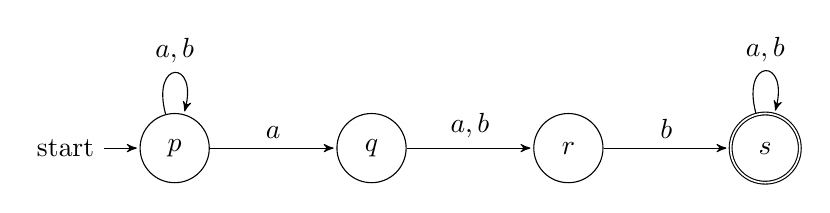
\begin{tikzpicture}[->,>=stealth',shorten >=1pt,auto,node distance=2.5cm]
  \node[initial, state]   (p)                {$p$};
  \node[state]            (q) [right of=p]  {$q$};
  \node[state]            (r) [right of=q]  {$r$};
  \node[state, accepting] (s) [right of=r]  {$s$};

  \path[->]
        (p) edge []  node [above] {$a$} (q)
             edge [loop above] node [above] {$a,b$} (p)
        (q) edge []  node [above] {$a,b$} (r)
        (r) edge [] node [above] {$b$} (s)
        (s) edge [loop above] node [above] {$a,b$} (s);
\end{tikzpicture}
\end{center}

Nicht erreichbare Zustände können weggelassen werden.

\begin{solutionorbox}

  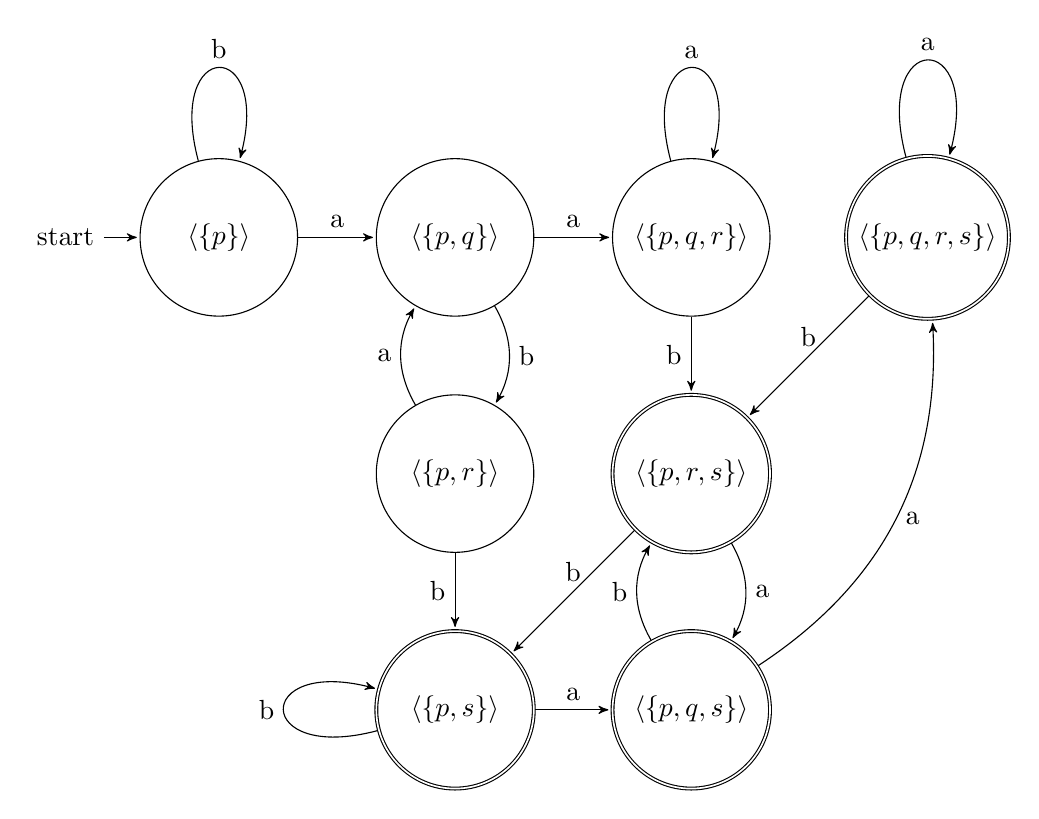
\begin{tikzpicture}[>=stealth', shorten >=1pt, auto, node distance=3cm, scale=1, transform shape, align=center, state/.style={circle, draw, minimum size=2cm}]
  \node[initial, state]   (p)                        {$\left<\{p\}\right>$};
  \node[state]            (p_q)     [right of=p]     {$\left<\{p,q\}\right>$};
  \node[state]            (p_r)     [below of=p_q]   {$\left<\{p,r\}\right>$};
  \node[state, accepting] (p_s)     [below of=p_r]   {$\left<\{p,s\}\right>$};
  \node[state]            (p_q_r)   [right of=p_q]   {$\left<\{p,q,r\}\right>$};
  \node[state, accepting] (p_r_s)   [below of=p_q_r] {$\left<\{p,r,s\}\right>$};
  \node[state, accepting] (p_q_s)   [below of=p_r_s] {$\left<\{p,q,s\}\right>$};
  \node[state, accepting] (p_q_r_s) [right of=p_q_r] {$\left<\{p,q,r,s\}\right>$};

  \path[->]
        (p)       edge              node [above] {a} (p_q)
                  edge [loop above] node [above] {b} (p)
        (p_q)     edge              node [above] {a} (p_q_r)
                  edge [bend left]  node [right] {b} (p_r)
        (p_r)     edge [bend left]  node [left]  {a} (p_q)
                  edge              node [left]  {b} (p_s)
        (p_s)     edge              node [above] {a} (p_q_s)
                  edge [loop left]  node [left]  {b} (p_s)
        (p_q_r)   edge [loop above] node [above] {a} (p_q_r)
                  edge              node [left]  {b} (p_r_s)
        (p_q_s)   edge [bend right] node [right] {a} (p_q_r_s)
                  edge [bend left]  node [left]  {b} (p_r_s)
        (p_r_s)   edge [bend left]  node [right] {a} (p_q_s)
                  edge              node [above] {b} (p_s)
        (p_q_r_s) edge [loop above] node [above] {a} (p_q_r_s)
                  edge              node [above] {b} (p_r_s)
        ;
\end{tikzpicture}

Die akzeptierenden Zustände könnten noch zusammengefasst werden (kurz begründen).
\end{solutionorbox}

\ifprintanswers
\newpage
\fi

\part Zeige, dass die folgende Sprache nicht regulär ist. Verwende eine
beliebige Methode, die in der Vorlesung vorgestellt wurde.

\begin{align*}
  L_3 &= \{0^{n(n+1)} \mid n \in \mathbb{N} \}
\end{align*}
\begin{solutionorbox}
      \begin{proof}[Beweis mittels Lemma 3.3] $ $\\
    Angenommen $L_3$ sei regulär.
    Es gibt also einen EA $A = (Q, \{0, 1\}, \hat{\delta}_A, q_0, F)$ mit $L(A) = L_3$.
    Beachten wir die Wörter
    \begin{align*}
      \lambda, 0, 0000, \dots , 0^{|Q|^2}
    \end{align*}
    Es existieren also $i, j \in \{1, 2, \dots, |Q|+1\}$ mit $i < j$
    und
    \begin{align*}
      \hat{\delta}_A(q_0, 0^{i^2}) &= \hat{\delta}_A(q_0, 0^{j^2})
    \end{align*}
    (Schubfachprinzip)\\
    Gemäss Lemma 3.3 im Buch gilt somit
    \begin{align*}
      0^{i^2} z \in L_3 &\iff 0^{j^2} z \in L_3
    \end{align*}
    für alle $z \in \{0, 1\}^*$. Für $z = 0^{i}$ haben wir aber einen Widerspruch,
        denn
        $0^{i^2} 0^{i} = 0^{i^2+i} \in L_3$ und $0^{j^2} 0^{i} \not\in L_3$,
        da $(j-1)j < j^2 \leq j^2 + i  < j(j+1)$.
        Das heisst also, dass
    $L_3$ nicht regulär ist.
      \end{proof}

      \hrule

      \begin{proof}[Mittels Pumping-Lemma:] $ $\\
        Angenommen $L_3$ sei regulär. Betrachten wir nun das Wort
        \begin{align*}
          w = 0^{n_0(n_0 + 1)}
        \end{align*}
        Offensichtlich gilt $|w| = n_0^2 + n_0 \geq n_0$.
        Folglich gibt es gemäss dem Pumping-Lemma, für das Wort $w$, eine Zerlegung
        $w = yxz$, wobei
        \begin{enumerate}[(i)]
          \item $|yx| \leq n_0$
          \item $|x| \geq 1$
          \item entweder $\{y x^k z \mid k \in \mathbb{N}\} \subseteq L_3$
            oder $\{y x^k z \mid k \in \mathbb{N}\} \cap L_3 = \emptyset$
        \end{enumerate}
        Nach (i) gibt es $y = 0^l$ und $x = 0^m$ für $l,m \in \mathbb{N}$
        mit $l+m \leq n_0$. Nach (ii) gilt $m \geq 1$. Und weil
        $w = 0^{n_0(n_0 + 1)} \in L_3$ ist, muss also
        $\{y x^k z \mid k \in \mathbb{N}\} \subseteq L_3$ gelten. Dies ist aber ein
        Widerspruch, da
        $yx^2z = 0^{n_0(n_0+1)+m} \not\in L_3$,
        weil $n_0(n_0 + 1) < n_0(n_0+1) + m < (n_0+1)(n_0 + 2)$.
        Somit ist
        $L_3 \not\in \mathcal{L}_{\mathrm{EA}}$
      \end{proof}

      \hrule

      \begin{proof}[Beweis mittels der Methode der Kolmogorov-Komplexität] $ $\\
        Angenommen, $L_3$ sei regulär. Für jedes $m \in \mathbb{N}$ ist $0^{2m+1}$
  das erste Wort in der Sprache
  \begin{align*}
    L_{0^{m(m+1)+1}} = \{y \mid 0^{m(m+1)+1}y \in L_3\}
  \end{align*}
        da $0^{m(m+1) + 1} 0^{2m+1} = 0^{m^2+ 3m + 2} = 0^{(m+1)(m+2)}$
Nach Satz 3.1 aus dem Buch existiert eine Konstante $c \in \mathbb{N}$,
unabhängig von $m$, so dass
  \begin{align*}
    K(0^{2m+1}) \leq \ceil{\log 2 (1 + 1)} + c = 1 + c
  \end{align*}
Da es nur endlich viele Programme der
konstanten Länge kleiner gleich $1 + c$ gibt, aber unendlich
viele Wörter der Form $0^{2m+1}$, ist dies ein Widerspruch. Also ist die Annahme falsch
und $L_3$ ist nicht regulär.
      \end{proof}
\end{solutionorbox}
  \end{parts}

  \question
  \begin{parts}
    \part Zeige $L_{\mathrm{H}}^C \leq_{\mathrm{R}} L_{\mathrm{diag}}$

    \textit{Zur Erinnerung:}

Sei $w_i$ das $i$-te Wort über $\{0,1\}$ und $M_i$ die $i$-te Turing-Maschine in
kanonischer Ordnung.
  \begin{align*}
    L_{\mathrm{diag}} &= \{w_i \in \{0,1\}^* \mid M_i \text{akzeptiert } w_i \text{ nicht}\} \\
    L_{\mathrm{H}}^C  &= \{\text{Kod}(M)\#w \in \{0,1, \#\}^* \mid
          M \text{ hält nicht auf } w\} \enspace \cup \\
          & \hspace{3em} \{x \in \{0,1, \#\}^* \mid x \text{ hat nicht die Form Kod}(M)\#w \}
  \end{align*}
\begin{solutionorbox}
  Wir zeigen $L_{\mathrm{H}}^C \leq_{\mathrm{EE}} L_{\mathrm{diag}}$ was
$L_{\mathrm{H}}^C \leq_{\mathrm{R}} L_{\mathrm{diag}}$ impliziert.

Wir beschreiben eine TM $M$, die $L_{\mathrm{H}}^C$ auf
$L_{\mathrm{diag}}$ reduziert. Für eine eingabe $x \in \{0,1, \#\}^*$ arbeit $M$ wie folgt:

  \begin{enumerate}
    \item Prüfe, ob $x$ die Form Kod$(M')\#w$ für eine TM $M'$ und ein Wort
      $w \in \{0,1\}^*$ hat.
      \begin{enumerate}[(i)]
    \item Falls nein: Konstruiere eine TM $M_\infty$ die immer in eine Endlosschleife geht.
    \item Falls ja: Modifiziere eine TM $M'$ zu einer TM $\overline{M}$ welche alle
      Transitionen von $q_{\mathrm{reject}}$ nach $q_{\mathrm{accept}}$ umleitet.
      Und konstruiere eine TM $\widehat{M}$, welche die Eingabe ignoriert und auf
      $w$ simuliert.
  \end{enumerate}
\item Berechne $w_i$ so, dass $M_i$ die konstruierte TM ist.

  Nun zeigen wir:
      \begin{align*}
      x \in L_{\mathrm{H}}^C \iff
      x \in L_{\mathrm{Diag}}
      \end{align*}

  Falls $x$ nicht die Form Kod$(M')\#w$ hat, gilt $x \in L_{\mathrm{H}}^C$ und \\
      $M_i = M_\infty$ hält nicht $\implies M_i$ akzeptiert $w_i$ nicht
      $\iff w_i \in L_{\mathrm{Diag}}$

      und sonst
      \begin{align*}
        x \not\in  L_{\mathrm{H}}^C &\iff M \text{ hält auf } w \\
         &\iff \overline{M} \text{ akzeptiert } w \\
         &\iff \widehat{M} = M_i \text{ akzeptiert alles, insbesonder } w_i \\
         &\iff M(x) = w_i \not\in L_{\mathrm{Diag}}
      \end{align*}
  \end{enumerate}
\end{solutionorbox}

    \part Zeige, dass $L_{\mathrm{diag}} \leq_{\mathrm{R}} L_{\mathrm{H}}$ gilt
\uplevel{\begin{solutionorbox}

  Um $L_{\mathrm{diag}} \leq_{\mathrm{R}} L_{\mathrm{H}}$ zu zeigen,
nehmen wir an, $A$ sei ein Algorithmus, der $L_H$ entscheidet. Dann
konstruieren wir einen Algorithmus $B$, der mit Hilfe von $A$ die Sprache
  $L_{\mathrm{diag}}$ entscheidet.
Der Algorithmus $B$ ist so strukturiert wie in der folgenden Abbildung gezeigt:

\tikzset{%
  block/.style    = {draw, thick, rectangle, minimum height = 3cm,
    minimum width = 1.5cm}}

  \begin{tikzpicture}[auto, thick, node distance=2.5cm, >=latex]
    \node[block]  (T) {$C$};
    \node[block, minimum width=2cm] [right of=T, xshift=1cm, align=center] (A) {$A$ \\ $L(A) = L_H$};
    \node[block, minimum height=2cm] [right =2.2cm of A.north, anchor=north west] (M) {M};
    
    \draw[->] ([yshift=8mm]T.east) -- ([yshift=8mm]A.west) node [midway] {$x=w_i$};
    \draw[->] ([yshift=-8mm]T.east) -- ([yshift=-8mm]A.west) node [midway] {\footnotesize Kod$(M_i)$};
    
    \draw[->] ([yshift=8mm]A.east) -- ([yshift=3mm]M.west) node [midway] {$\in L_H$};
    \draw[->] ([yshift=-8mm]A.east) -- (9,-8mm) node [near start, below] {$\not\in L_H$}
               -- (9,2mm);
    
    \draw[->] ([yshift=5mm]M.east) -- (10, 10mm) node [midway] {\footnotesize$w_i \in L(M_i)$};
    \draw[->] ([yshift=-3mm]M.east) -- (10,2mm) node [midway] {\footnotesize$w_i \not\in L(M_i)$};
    
    \draw[->] (10, 10mm) -- (12, 10mm) node [midway] {\footnotesize$x \not\in L_{diag}$};
    \draw[->] (10,2mm) -- (12,2mm) node [midway] {\footnotesize$x \in L_{diag}$};
    \draw[->] (-3,0) -- (T.west) node [near start] {\footnotesize$x \in \Sigma^*$};
	\draw (-1.5cm,-2cm) rectangle (10cm,2cm);
  \end{tikzpicture}

  Für eine Eingabe $x \in \Sigma^*_{\mathrm{bool}}$ berechnet das
  Teilprogramm $C$ das $i \in \mathbb{N}$, so dass $x = w_i$ das
  $i$-te Wort über $\Sigma_{\mathrm{bool}}$ in
  kanonischer Ordnung ist, und die Kodierung Kod$(M_i)$ der $i$-ten
  TM. Das Teilprogramm $A$ für $L_{\mathrm{H}}$ bekommt Kod$(M_i)$ und
  $x = w_i$ als Eingabe in der Form
  Kod$(M_i)\#x$.
  Falls $A$ die Eingabe Kod$(M_i)\#x$ verwirft,
  dann hält $M_i$ nicht auf $w_i$, also akzeptiert $M_i$
  das Wort $w_i$ auch nicht.
  Also gilt $w_i \in L_{\mathrm{diag}}$ und $B$ akzeptiert seine Eingabe $x = w_i$.
  Falls $A$ die Eingabe
  Kod$(M_i)\#x$ akzeptiert, dann hält $M_i$ auf $w_i$. In diesem Fall simuliert
  das Teilprogramm $M$ die Arbeit von $M_i$ auf $w_i$. Diese Simulation endet auf jeden Fall
  in endlicher Zeit. Falls die Simulation ergibt, dass $M_i$ das Wort $w_i$
  akzeptiert, dann gilt
  $w_i \in L_{diag}$ und $B$ verwirft seine Eingabe $x = w_i$. Sonst verwirft $M_i$
  das Wort $w_i$, es gilt
  also $w_i \in L_{\mathrm{diag}}$ und $B$ akzeptiert seine Eingabe $x = w_i$.
\end{solutionorbox}}
  \end{parts}

\end{questions}

\end{document}
